\documentclass[11pt]{article}
\usepackage[margin=1in]{geometry}
\usepackage[T1]{fontenc}
\usepackage[utf8]{inputenc}
\usepackage{lmodern}
\usepackage{microtype}
\usepackage{amsmath}
\usepackage{booktabs}
\usepackage{multirow}
\usepackage{xcolor}
\usepackage{tikz}
\usepackage{graphicx}
\usepackage{enumitem}
\usepackage[numbers,sort&compress]{natbib}
\usepackage[colorlinks=true,linkcolor=blue!50!black,citecolor=blue!50!black,urlcolor=blue!50!black]{hyperref}
\usepackage{url}

\setlist{itemsep=2pt,topsep=4pt}
\newcommand{\todo}[1]{\textcolor{red}{\textbf{[TODO: #1]}}}
\newcommand{\ci}[2]{\,[#1,\,#2]}
\newcommand{\code}[1]{\texttt{#1}}

\title{Format or Presence? Measuring Citation Survival\\When Agents Consume Retrieval over MCP}
\author{Md Ayan Arshad\\Independent researcher\\\texttt{ayanarshad2002@gmail.com}}
\date{}

\begin{document}
\maketitle

\begin{abstract}
Retrieval providers increasingly serve their knowledge to third-party agents through the Model
Context Protocol (MCP): the server returns chunks tagged with source URLs, and an agent the
provider does not control writes the final answer. Whether that answer still cites its sources is
unmeasured. We introduce Citation Survival Rate (CSR), which asks, of the gold sources an agent
actually retrieved, how many end up cited on a claim the cited source supports, combining an
entailment-based support check with a check against the logged tool-call trace. On 127
hand-verified questions over the FastAPI documentation, served by a self-hosted MCP server that
mirrors a commercial retrieval contract, a single-shot RAG pipeline and a LangGraph agent cite
equally well (CSR 0.618 and 0.614 with gpt-4o-mini), while an OpenAI Agents SDK agent with the same
model and prompt scores 0.323. That gap is mostly not lost citations: the SDK agent ignores the
requested \code{[url]} format in 51 of 127 answers and cites with Markdown links instead
(single-shot: 0). A pre-registered ablation traces this format drift to the model API the SDK
calls by default: switching from the Responses API to Chat Completions cuts wrong-format answers
from 41 to 9. Three runs per setup show the drift in every run (46--53 answers) and a smaller
residual loss of citations, robust under both an NLI scorer and a gpt-4o judge ($-0.12$ and
$-0.09$ CSR, about a third of the apparent gap) and not detectable at temperature 0. Giving each
chunk a short source ID at the tool contract, and mapping IDs back to URLs after the answer is
written, cuts wrong-format answers to 4--5 per run, raises the SDK agent's CSR by 0.10--0.13 and
closes its gap to single-shot.
We validate CSR against blind human judgement (25--27 of 30 units agree, depending on the
scorer), and report two failures of our own evaluation that would have produced false findings: a
format-strict citation parser that turned format drift into an apparent 50\% citation loss, and a
citation guardrail whose precision looked high under the model that built it and was 30\% under a
blind human audit. Code, data, traces and human labels are released.
\end{abstract}

% ---------------------------------------------------------------------------
\section{Introduction}

Retrieval-augmented generation (RAG) \citep{lewis2020rag} is usually evaluated on whether answers
are correct. For documentation assistants, attribution matters as much: an answer that is right
but uncited cannot be checked, and it hides the source a user would click through to. Citation
quality has well-established metrics for the single-shot setting, where one system retrieves and
writes the answer \citep{gao2023alce,liu2023verifiability,rashkin2023ais}.

That setting is changing. Through the Model Context Protocol (MCP) \citep{mcp2026spec}, a
retrieval provider exposes a search tool, and a customer's agent calls it, possibly many times,
and writes the answer itself. The provider controls what it returns, typically chunks of the form
\code{\{source\_url, content\}}, but not the framework, model, prompt or settings of the agent on the
other side. If attribution degrades there, the provider cannot see it.

We ask a narrow question: \emph{when the same model, prompt and retrieval server are used, do
citations survive the trip through an agent framework as well as they do in single-shot RAG?} We
make five contributions.

\begin{enumerate}
\item \textbf{A metric.} Citation Survival Rate (CSR) conditions on retrieval, so it separates
attribution failures from retrieval failures, and combines a support check with a trace-grounding
check (\S\ref{sec:csr}). We report it in two views: counting only the requested citation format,
and counting any link format.
\item \textbf{A controlled benchmark.} 127 hand-verified questions, a self-hosted MCP server that
mirrors a published commercial contract, and three pipelines (single-shot, LangGraph, OpenAI
Agents SDK) with identical prompts, on gpt-4o-mini and Claude Sonnet 4.6 (\S\ref{sec:setup}).
\item \textbf{Findings.} With the OpenAI Agents SDK, most of the apparent citation loss is
\emph{format drift}, which a pre-registered ablation ties to the SDK's default model API; across
three runs a smaller loss of citations remains (\S\ref{sec:results}).
\item \textbf{A fix at the tool contract.} Short source IDs returned by the retrieval server
remove most of the drift and close the gap, with no change on the agent's side beyond its
citation instruction (\S\ref{sec:v3a}).
\item \textbf{A methodological record.} The metric agrees with blind human judgement, and we
document two evaluation failures we caught in our own pipeline, including one that reached a
public draft (\S\ref{sec:lessons}).
\end{enumerate}

% ---------------------------------------------------------------------------
\section{Related work}

\paragraph{Citation evaluation.} ALCE \citep{gao2023alce} measures citation recall and precision
with an NLI model \citep{honovich2022true}; AIS \citep{rashkin2023ais} defines attribution to
identified sources; \citet{liu2023verifiability} audit generative search engines and find many
statements unsupported by their citations; attributed QA \citep{bohnet2022attributed} frames
attribution as part of the task. These works evaluate a system that both retrieves and writes.
We use ALCE-style entailment and FActScore-style atomic claims \citep{min2023factscore}, and move
the question to the boundary between a retrieval server and an independent agent.

\paragraph{Citations in agents.} Recent work studies citations produced by agents rather than
single-shot systems: localising faithfulness and citation mistakes across the agents of a deep
research system \citep{hirsch2026blame}, parsing and verifying the inline citations of deep
research reports \citep{onweller2026cited}, and detecting hallucinated references in commercial
models and agents \citep{rao2026reference}. We isolate a narrower variable: the same model, prompt
and retrieval server, with only the agent framework (and its settings) changed.

\paragraph{Correct is not faithful.} \citet{wallat2025correctness} show that a citation can be
correct (the source supports the claim) without being faithful (the model did not actually use
it), and test faithfulness by counterfactual regeneration. We take the concept, not the method:
our trace-grounding check is a cheap necessary condition (the cited source must have been
retrieved), not a causal test.

\paragraph{Fact-checking models and LLM judges.} MiniCheck \citep{tang2024minicheck} checks claims
against grounding documents at low cost; LLM-as-a-judge \citep{zheng2023judging} is common for
open-ended evaluation. We compare such checkers against human labels before choosing one
(\S\ref{sec:validation}).

\paragraph{Format following.} Instruction-following benchmarks measure compliance with explicit
format constraints \citep{zhou2023ifeval}; format restrictions interact with task quality
\citep{tam2024speakfreely}; and evaluation outcomes can hinge on surface formatting
\citep{sclar2024quantifying}. Our main finding is an instance of format non-compliance with a
practical cost: anything that parses citations by format loses them.

% ---------------------------------------------------------------------------
\section{Citation Survival Rate}
\label{sec:csr}

Each answer is split into units: a span of text and the citations attached to it. Each unit is
decomposed into atomic claims \citep{min2023factscore} by gpt-4o-mini at temperature 0 (cached, and
identical for every pipeline and scorer). Two checks follow.

\begin{enumerate}
\item \textbf{Support.} A claim is supported if the concatenated text of the chunks its unit cites
entails it. The reference scorer is \code{cross-encoder/nli-deberta-v3-base}
\citep{he2023debertav3} with argmax $=$ entailment; \S\ref{sec:validation} adds an LLM judge.
\item \textbf{Trace grounding.} A cited URL counts only if it appears in the chunks the pipeline
actually retrieved, according to the logged tool-call trace.
\end{enumerate}

Let $G$ be the gold source URLs of a question and $R$ the URLs retrieved across all of the agent's
tool calls. A gold URL $g \in G \cap R$ \emph{survives} if at least one unit cites $g$ and has at
least one supported claim. Then
\[
\mathrm{CSR} = \frac{|\{g \in G \cap R : g \text{ survives}\}|}{|G \cap R|},
\]
undefined (not zero) when $G \cap R = \emptyset$. Conditioning on $G \cap R$ means a pipeline is not
penalised for retrieval failures, only for losing what it retrieved. We report the mean over
questions where CSR is defined.

\paragraph{Two views of ``cited''.} The prompt asks for \code{[url]} immediately after each claim.
In the \emph{requested-format} view only that form is a citation. In the \emph{any-format} view,
\code{[url]}, Markdown links \code{[text](url)}, and the bracketed form \code{[[title](url)]} all
count; bare URLs in running text do not, because their attachment to a claim is ambiguous. The
requested-format view measures compliance and attribution together; the any-format view measures
whether sources are cited at all. The any-format rule was fixed and recorded before re-scoring.

% ---------------------------------------------------------------------------
\section{Experimental setup}
\label{sec:setup}

\paragraph{Corpus and server.} The FastAPI documentation (raw Markdown from its repository; 153
pages) is split at Markdown headings into 2,085 chunks, embedded with
\code{text-embedding-3-small}, and stored in Chroma. A FastMCP server exposes one tool,
\code{search\_fastapi\_knowledge\_sources}, over streamable HTTP, returning
\code{\{source\_url, content\}} objects in relevance order (top 15, at most 35,000 characters). The
tool name, result shape and limits mirror the documented contract of a commercial retrieval
provider's hosted MCP server \citep{kapa2025mcp}; it is a mirror, not that production system.

\paragraph{Questions.} About 250 candidate questions with gold URLs were drafted by gpt-4o-mini from
the corpus; the author verified each question and gold attribution by hand against the live
documentation and kept 127: 82 single-source, 29 multi-source and 16 unanswerable.

\paragraph{Pipelines.} All three use the same citation instructions, asking for
\code{[source\_url]} immediately after every factual claim; the two agents share one system prompt
word for word (Appendix~\ref{app:prompts}).
\begin{itemize}
\item \textbf{Single-shot RAG}: one retrieval call through the MCP server with the question, one
generation, temperature 0.
\item \textbf{LangGraph agent}: a ReAct agent \citep{yao2023react} built with
\code{create\_react\_agent} and \code{langchain-mcp-adapters}, following the retrieval provider's
published example; temperature 0; at most 10 turns.
\item \textbf{OpenAI Agents SDK agent}: \code{Agent} with \code{MCPServerStreamableHttp}, following
the SDK's MCP documentation \citep{openai2025agentssdk}; at most 10 turns. In the published
configuration temperature is left unset, as in the SDK's defaults.
\end{itemize}
Models: gpt-4o-mini for all three; Claude Sonnet 4.6 (via Amazon Bedrock) for single-shot and
LangGraph. Versions are pinned (\code{openai-agents} 0.17.7, \code{langgraph} 1.2.6,
\code{langchain-mcp-adapters} 0.3.0, \code{fastmcp} 3.4.2).

\paragraph{Statistics.} All pipelines answer the same questions, so differences are tested with a
paired bootstrap over per-question CSR differences \citep{efron1993bootstrap} (10,000 resamples,
seed 42, 95\% percentile intervals). We call a difference significant when its interval excludes
zero. Agreement with humans is reported with Cohen's $\kappa$ \citep{cohen1960kappa} and proportions
with Wilson intervals \citep{wilson1927probable}.

% ---------------------------------------------------------------------------
\section{Results}
\label{sec:results}

\subsection{Headline: a large gap in one view, a small one in the other}

\begin{table}[t]
\centering
\small
\begin{tabular}{llcccc}
\toprule
& & \multicolumn{2}{c}{Requested format} & \multicolumn{2}{c}{Any format} \\
\cmidrule(lr){3-4}\cmidrule(lr){5-6}
Pipeline & Model & DeBERTa & gpt-4o judge & DeBERTa & gpt-4o judge \\
\midrule
Single-shot & gpt-4o-mini & 0.618 & 0.665 & 0.618 & 0.665 \\
LangGraph & gpt-4o-mini & 0.614 & 0.700 & 0.643 & 0.729 \\
OpenAI Agents SDK & gpt-4o-mini & 0.323 & 0.379 & 0.470 & 0.571 \\
\midrule
Single-shot & Claude Sonnet 4.6 & 0.774 & 0.887 & 0.774 & 0.887 \\
LangGraph & Claude Sonnet 4.6 & 0.710 & 0.804 & 0.710 & 0.804 \\
\bottomrule
\end{tabular}
\caption{Mean CSR, 127 questions (CSR defined on 99--107 per pipeline). Bootstrap 95\% intervals
are about $\pm0.09$ (full table in the released results). The SDK $\times$ Claude combination was
not run.}
\label{tab:headline}
\end{table}

\begin{table}[t]
\centering
\small
\begin{tabular}{lcc}
\toprule
Paired difference (B $-$ A) & Requested format & Any format \\
\midrule
SDK $-$ single-shot (DeBERTa) & $-0.311$\ci{-0.434}{-0.189} & $-0.163$\ci{-0.281}{-0.046} \\
SDK $-$ single-shot (judge) & $-0.296$\ci{-0.413}{-0.179} & $-0.102$\ci{-0.214}{+0.010} \\
SDK, temperature 0 $-$ single-shot (DeBERTa) & $-0.207$\ci{-0.313}{-0.101} & $-0.056$\ci{-0.162}{+0.051} \\
SDK, temperature 0 $-$ single-shot (judge) & $-0.227$\ci{-0.338}{-0.121} & $-0.045$\ci{-0.152}{+0.061} \\
LangGraph $-$ single-shot, gpt-4o-mini (DeBERTa) & $+0.000$\ci{-0.093}{+0.093} & $+0.029$\ci{-0.064}{+0.123} \\
LangGraph $-$ single-shot, gpt-4o-mini (judge) & $+0.029$\ci{-0.044}{+0.108} & $+0.059$\ci{-0.020}{+0.137} \\
LangGraph $-$ single-shot, Claude (DeBERTa) & $-0.077$\ci{-0.168}{+0.014} & $-0.077$\ci{-0.168}{+0.014} \\
LangGraph $-$ single-shot, Claude (judge) & $-0.096$\ci{-0.178}{-0.019} & $-0.096$\ci{-0.178}{-0.019} \\
\bottomrule
\end{tabular}
\caption{Paired bootstrap differences in CSR with 95\% intervals (published run of each setup).}
\label{tab:paired}
\end{table}

Tables~\ref{tab:headline} and~\ref{tab:paired} give the main result. Counting only the requested
format, the OpenAI Agents SDK agent scores about 0.3 below single-shot under both scorers. Counting
any link format, the gap is $-0.163$ under DeBERTa (significant) and $-0.102$ under the judge (not
significant). With the SDK set to temperature 0, the any-format gap is small and not significant
under either scorer. The LangGraph agent matches single-shot on gpt-4o-mini in every view. On
Claude, LangGraph is lower by 0.08--0.10, significant only under the judge.

So the agent loop itself does not cost citations, and most of the SDK's apparent loss is format.
From this single run, whether a residual loss exists depends on the scorer. Three runs per setup
settle it (\S\ref{sec:repeats}): a residual loss of about 0.09--0.12 is robust under both scorers
with the SDK's defaults, and not detectable at temperature 0.

\subsection{What the SDK agent does instead}

\begin{table}[t]
\centering
\small
\begin{tabular}{lcccc}
\toprule
Run (gpt-4o-mini) & Requested & Other link format & Bare URL only & No URL \\
\midrule
Single-shot & 108 & \textbf{0} & 0 & 19 \\
LangGraph & 112 & \textbf{8} & 1 & 6 \\
SDK, defaults (published run) & 61 & \textbf{51} & 7 & 8 \\
\midrule
E1: SDK, temperature 0 & 73 & \textbf{41} & 2 & 11 \\
E2: E1 + provider's tool description & 73 & \textbf{41} & 2 & 11 \\
E3: E1 + Chat Completions API & 109 & \textbf{9} & 0 & 9 \\
E4: E1 + provider's full setup$^\dagger$ & 84 & \textbf{20} & 6 & 17 \\
\bottomrule
\end{tabular}
\caption{Citation format per answer (127 answers per run; each answer in exactly one bucket; no
scorer involved). ``Requested'': at least one citation in the requested format. $^\dagger$E4 asks
for \code{[[title](url)]}, so for E4 that is the requested format and \code{[url]} counts as
``other''. ``No URL'' includes legitimate ``the documentation does not say'' answers.}
\label{tab:format}
\end{table}

Table~\ref{tab:format} counts formats directly. Single-shot never cites in an unrequested link
format; the SDK agent does so in 51 of 127 answers, writing per-claim Markdown links
(\code{[Path Parameters](https://fastapi.tiangolo.com/tutorial/path-params/)}) where the prompt asks
for \code{[https://fastapi.tiangolo.com/tutorial/path-params/]}. These links are mostly real
citations: in the published run, 98 of the 118 Markdown links in answers without any
\code{[url]} point to a page the agent retrieved. Logging the exact model inputs shows every chunk
reaches the model with its \code{source\_url} intact; the drift happens while writing the answer.

\subsection{A pre-registered ablation of the SDK}
\label{sec:ablation}

To find the cause we changed one setting at a time, with the plan and the success criterion
recorded before running: E1 sets temperature to 0; E2 adds the retrieval provider's recommended
tool description \citep{kapa2025promptagent}; E3 switches the SDK from OpenAI's Responses API (its
default \citep{openai2025responses}) to Chat Completions, which the LangGraph agent uses; E4 adds the
provider's full recommended setup (system prompt, tool description and its \code{[[title](url)]}
citation format). E0 re-runs the defaults.

\begin{itemize}
\item \textbf{The API, not the loop or the temperature, drives the drift.} Chat Completions cuts
wrong-format answers from 41 to 9 (E3 vs E1), close to LangGraph's 8.
\item \textbf{A tool description alone does nothing} (E2: identical format counts; CSR
$-0.040$, not significant), consistent with the provider's guidance placing citation rules in the
system prompt. The full setup (E4) cuts wrong-format answers from 41 to 20.
\item \textbf{None of these changes alters citation presence.} In the any-format view, E3 vs E1 is
$+0.020$ (DeBERTa) / $+0.069$ (judge) and E4 vs E1 $+0.030$ / $+0.035$, none significant. In the
requested-format view the same comparisons were $+0.108$ / $+0.201$ and $+0.111$ / $+0.136$, all
significant: those gains were format.
\end{itemize}

We do not know why the Responses API path produces more Markdown links; we only establish that it
does, on this model and SDK version.

\subsection{Repeat runs}
\label{sec:repeats}

Every result above is one run per setup. Bootstrap intervals cover question sampling, not
run-to-run variation in generation. We therefore repeated each gpt-4o-mini setup twice more with
fresh, uncached generations (no seed is available for the SDK, so these are repeats, not seeded
runs), with a decision rule recorded in advance: a CSR difference is robust only if it has the
same sign in all three runs and the paired interval on per-question CSR averaged over runs excludes
zero; a format difference is robust only if it has the same direction in all three runs.

\begin{table}[t]
\centering
\small
\begin{tabular}{lccc}
\toprule
Setup (gpt-4o-mini) & Run 1 & Run 2 & Run 3 \\
\midrule
Single-shot & 0 & 0 & 0 \\
LangGraph & 8 & 12 & 9 \\
SDK, defaults & 51 & 53 & 46 \\
E1: SDK, temperature 0 & 41 & 60 & 60 \\
E3: E1 + Chat Completions & 9 & 12 & 15 \\
E4: E1 + provider's full setup & 20 & 23 & 16 \\
\midrule
v3a: SDK + source IDs & 5 & 5 & 4 \\
v3a: LangGraph + source IDs & 0 & 1 & 5 \\
\bottomrule
\end{tabular}
\caption{Format drift per run: answers citing only in a link format other than the one requested
(out of 127). Run 1 is the published run. E0, an earlier re-run of the SDK defaults, had 38.}
\label{tab:drift-runs}
\end{table}

\begin{table}[t]
\centering
\small
\resizebox{\linewidth}{!}{%
\begin{tabular}{llccc}
\toprule
Comparison (B $-$ A) & View, scorer & Runs 1 / 2 / 3 & Pooled [95\% CI] & Verdict \\
\midrule
\multirow{3}{*}{SDK defaults $-$ single-shot} & requested, DeBERTa & $-.311$ / $-.311$ / $-.285$ & $-0.302$\ci{-0.394}{-0.210} & robust \\
& any, DeBERTa & $-.163$ / $-.143$ / $-.055$ & $-0.120$\ci{-0.209}{-0.030} & robust \\
& any, judge & $-.102$ / $-.087$ / $-.045$ & $-0.086$\ci{-0.164}{-0.005} & robust \\
\midrule
\multirow{2}{*}{SDK temp.\ 0 $-$ single-shot} & any, DeBERTa & $-.056$ / $-.100$ / $-.051$ & $-0.066$\ci{-0.160}{+0.028} & not robust \\
& any, judge & $-.045$ / $-.050$ / $-.040$ & $-0.045$\ci{-0.130}{+0.043} & not robust \\
\midrule
\multirow{2}{*}{LangGraph $-$ single-shot} & any, DeBERTa & $+.029$ / $+.000$ / $+.044$ & $+0.023$\ci{-0.062}{+0.105} & not robust \\
& any, judge & $+.059$ / $+.034$ / $+.034$ & $+0.037$\ci{-0.036}{+0.110} & not robust \\
\bottomrule
\end{tabular}}
\caption{Paired CSR differences across three runs. ``Pooled'': per-question CSR averaged over the
three runs of each setup, then paired bootstrap. Robust (pre-registered): same sign in every run
and pooled interval excluding zero.}
\label{tab:repeats}
\end{table}

\begin{figure}[t]
\centering
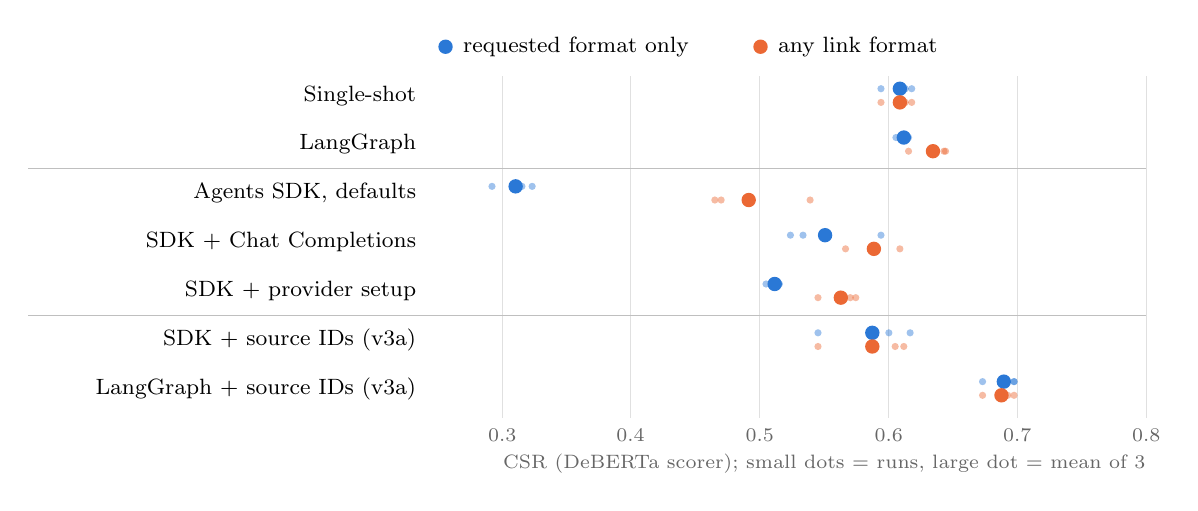
\begin{tikzpicture}[x=1cm, y=-0.62cm]
\definecolor{reqcol}{HTML}{2A78D6}\definecolor{anycol}{HTML}{EB6834}
\draw[black!12] (0.82,-0.4) -- (0.82,6.60);
\node[font=\scriptsize,text=black!60] at (0.82,6.95) {0.3};
\draw[black!12] (2.45,-0.4) -- (2.45,6.60);
\node[font=\scriptsize,text=black!60] at (2.45,6.95) {0.4};
\draw[black!12] (4.09,-0.4) -- (4.09,6.60);
\node[font=\scriptsize,text=black!60] at (4.09,6.95) {0.5};
\draw[black!12] (5.73,-0.4) -- (5.73,6.60);
\node[font=\scriptsize,text=black!60] at (5.73,6.95) {0.6};
\draw[black!12] (7.36,-0.4) -- (7.36,6.60);
\node[font=\scriptsize,text=black!60] at (7.36,6.95) {0.7};
\draw[black!12] (9.00,-0.4) -- (9.00,6.60);
\node[font=\scriptsize,text=black!60] at (9.00,6.95) {0.8};
\node[font=\scriptsize,text=black!60] at (4.91,7.55) {CSR (DeBERTa scorer); small dots = runs, large dot = mean of 3};
\node[anchor=east,font=\footnotesize] at (-0.15,0) {Single-shot};
\fill[reqcol,opacity=0.45] (6.02,-0.14) circle (1.3pt);
\fill[reqcol,opacity=0.45] (5.94,-0.14) circle (1.3pt);
\fill[reqcol,opacity=0.45] (5.63,-0.14) circle (1.3pt);
\fill[reqcol] (5.87,-0.14) circle (2.6pt);
\fill[anycol,opacity=0.45] (6.02,0.14) circle (1.3pt);
\fill[anycol,opacity=0.45] (5.94,0.14) circle (1.3pt);
\fill[anycol,opacity=0.45] (5.63,0.14) circle (1.3pt);
\fill[anycol] (5.87,0.14) circle (2.6pt);
\node[anchor=east,font=\footnotesize] at (-0.15,1) {LangGraph};
\fill[reqcol,opacity=0.45] (5.96,0.86) circle (1.3pt);
\fill[reqcol,opacity=0.45] (5.82,0.86) circle (1.3pt);
\fill[reqcol,opacity=0.45] (5.98,0.86) circle (1.3pt);
\fill[reqcol] (5.92,0.86) circle (2.6pt);
\fill[anycol,opacity=0.45] (6.43,1.14) circle (1.3pt);
\fill[anycol,opacity=0.45] (5.98,1.14) circle (1.3pt);
\fill[anycol,opacity=0.45] (6.45,1.14) circle (1.3pt);
\fill[anycol] (6.29,1.14) circle (2.6pt);
\node[anchor=east,font=\footnotesize] at (-0.15,2) {Agents SDK, defaults};
\draw[black!25] (-5.2,1.5) -- (9.00,1.5);
\fill[reqcol,opacity=0.45] (1.20,1.86) circle (1.3pt);
\fill[reqcol,opacity=0.45] (0.69,1.86) circle (1.3pt);
\fill[reqcol,opacity=0.45] (1.07,1.86) circle (1.3pt);
\fill[reqcol] (0.99,1.86) circle (2.6pt);
\fill[anycol,opacity=0.45] (3.60,2.14) circle (1.3pt);
\fill[anycol,opacity=0.45] (3.52,2.14) circle (1.3pt);
\fill[anycol,opacity=0.45] (4.73,2.14) circle (1.3pt);
\fill[anycol] (3.95,2.14) circle (2.6pt);
\node[anchor=east,font=\footnotesize] at (-0.15,3) {SDK + Chat Completions};
\fill[reqcol,opacity=0.45] (4.64,2.86) circle (1.3pt);
\fill[reqcol,opacity=0.45] (5.63,2.86) circle (1.3pt);
\fill[reqcol,opacity=0.45] (4.48,2.86) circle (1.3pt);
\fill[reqcol] (4.92,2.86) circle (2.6pt);
\fill[anycol,opacity=0.45] (5.57,3.14) circle (1.3pt);
\fill[anycol,opacity=0.45] (5.87,3.14) circle (1.3pt);
\fill[anycol,opacity=0.45] (5.18,3.14) circle (1.3pt);
\fill[anycol] (5.54,3.14) circle (2.6pt);
\node[anchor=east,font=\footnotesize] at (-0.15,4) {SDK + provider setup};
\fill[reqcol,opacity=0.45] (4.33,3.86) circle (1.3pt);
\fill[reqcol,opacity=0.45] (4.17,3.86) circle (1.3pt);
\fill[reqcol,opacity=0.45] (4.34,3.86) circle (1.3pt);
\fill[reqcol] (4.28,3.86) circle (2.6pt);
\fill[anycol,opacity=0.45] (5.31,4.14) circle (1.3pt);
\fill[anycol,opacity=0.45] (5.24,4.14) circle (1.3pt);
\fill[anycol,opacity=0.45] (4.83,4.14) circle (1.3pt);
\fill[anycol] (5.12,4.14) circle (2.6pt);
\node[anchor=east,font=\footnotesize] at (-0.15,5) {SDK + source IDs (v3a)};
\draw[black!25] (-5.2,4.5) -- (9.00,4.5);
\fill[reqcol,opacity=0.45] (6.00,4.86) circle (1.3pt);
\fill[reqcol,opacity=0.45] (4.83,4.86) circle (1.3pt);
\fill[reqcol,opacity=0.45] (5.73,4.86) circle (1.3pt);
\fill[reqcol] (5.52,4.86) circle (2.6pt);
\fill[anycol,opacity=0.45] (5.92,5.14) circle (1.3pt);
\fill[anycol,opacity=0.45] (4.83,5.14) circle (1.3pt);
\fill[anycol,opacity=0.45] (5.81,5.14) circle (1.3pt);
\fill[anycol] (5.52,5.14) circle (2.6pt);
\node[anchor=east,font=\footnotesize] at (-0.15,6) {LangGraph + source IDs (v3a)};
\fill[reqcol,opacity=0.45] (6.92,5.86) circle (1.3pt);
\fill[reqcol,opacity=0.45] (7.32,5.86) circle (1.3pt);
\fill[reqcol,opacity=0.45] (7.32,5.86) circle (1.3pt);
\fill[reqcol] (7.19,5.86) circle (2.6pt);
\fill[anycol,opacity=0.45] (6.92,6.14) circle (1.3pt);
\fill[anycol,opacity=0.45] (7.24,6.14) circle (1.3pt);
\fill[anycol,opacity=0.45] (7.32,6.14) circle (1.3pt);
\fill[anycol] (7.16,6.14) circle (2.6pt);
\fill[reqcol] (0.10,-1.0) circle (2.6pt);
\node[anchor=west,font=\footnotesize] at (0.20,-1.0) {requested format only};
\fill[anycol] (4.10,-1.0) circle (2.6pt);
\node[anchor=west,font=\footnotesize] at (4.20,-1.0) {any link format};
\end{tikzpicture}

\caption{CSR per run for each setup, counting only the requested format (blue) and any link format
(orange), reference DeBERTa scorer. The gap between the two colours is format; the remaining
distance from single-shot is loss of citations.}
\label{fig:csr}
\end{figure}

Table~\ref{tab:drift-runs} and Figure~\ref{fig:csr} show the result.

\begin{itemize}
\item \textbf{The format drift replicates.} The SDK agent cites in an unrequested format in 46--53
answers per run; single-shot never does. Chat Completions (E3) and the provider's full setup (E4)
cut it in every run. Temperature 0 does not: E1 drifted more than the defaults in runs 2 and 3.
\item \textbf{A smaller loss of citations is also real.} The any-format gap between the SDK's
defaults and single-shot has the same sign in all three runs and a pooled interval excluding zero
under both scorers (Table~\ref{tab:repeats}): $-0.120$ (DeBERTa) and $-0.086$ (judge), against
$-0.302$ in the requested-format view. Roughly two thirds of the apparent loss is format and one
third is citations not given at all. The per-run gap ranges from $-0.05$ to $-0.16$, which is why a
single run could not settle it.
\item \textbf{At temperature 0 there is no detectable loss}, and LangGraph matches single-shot in
every run and view.
\end{itemize}

% ---------------------------------------------------------------------------
\section{Is CSR trustworthy?}
\label{sec:validation}

\paragraph{Which support checker agrees with humans?} We collected 115 blind human judgements of
whether a chunk supports a sentence (50 development, 65 held-out), and compared checkers
(Table~\ref{tab:verifiers}). Every sampled pair had been accepted by DeBERTa at sampling time, so
the benchmark measures how well each checker rejects DeBERTa's false positives. On the held-out
set the gpt-4o judge, using the same rubric as the human labeller, agreed best ($\kappa = 0.86$).
Removing Markdown and code from the input helped every model. We use the gpt-4o judge as the
independent scorer, and MiniCheck, a different model, as the verifier inside the guardrail, so the
guardrail never grades its own work.

\begin{table}[t]
\centering
\small
\begin{tabular}{lcccc}
\toprule
Checker (held-out, $n=65$, default decision rules) & Precision & Recall & Accuracy & $\kappa$ \\
\midrule
DeBERTa NLI, raw text & 0.75 & 0.70 & 0.65 & 0.24 \\
DeBERTa NLI, cleaned prose, claims & 0.78 & 0.91 & 0.77 & 0.44 \\
MiniCheck-Flan-T5-Large, cleaned prose & 0.90 & 0.84 & 0.83 & 0.63 \\
\quad + code-symbol check & 0.92 & 0.84 & 0.85 & 0.67 \\
Claude Sonnet 4.6 judge & 0.97 & 0.74 & 0.82 & 0.63 \\
gpt-4o judge & 0.95 & 0.95 & 0.94 & 0.86 \\
\bottomrule
\end{tabular}
\caption{Support checkers against blind human labels (strict gold: only ``correct'' counts as
support). Thresholds tuned on the development set did not transfer and are not used.}
\label{tab:verifiers}
\end{table}

\paragraph{Does CSR agree with a human?} We sampled 30 CSR units (a gold source the pipeline
retrieved; 6 per pipeline) and asked, blind to scores, whether that source survived, correctly
cited. Agreement was 25/30 for DeBERTa ($\kappa = 0.64$), 27/30 for the gpt-4o judge
($\kappa = 0.77$) and 26/30 for a Claude judge ($\kappa = 0.70$). Errors run mostly one way:
scorers miss support a human sees, so absolute CSR is, if anything, conservative. One caveat
belongs to \S\ref{sec:lessons}: the labelling page recognised only \code{[url]}, so on 2 of the 30
units (both SDK) human and scorers agreed that a source was uncited when it was in fact cited as a
Markdown link.

\paragraph{Does a conclusion depend on the scorer?} Absolute CSR does: the judges score
0.03--0.11 higher than DeBERTa in every pipeline. The format result and the LangGraph result hold
under every scorer; the SDK's any-format gap does not. All scorers share one citation parser, so
agreement between scorers says nothing about citation format; this is why we report both views.

% ---------------------------------------------------------------------------
\section{Putting citations back}
\label{sec:guardrail}

A retrieval provider controls what happens at its boundary, so we also tested repair: middleware
that adds citations to an agent's answer. It may only insert citation tokens; a check that the
answer is byte-identical once citations are stripped runs on every answer.

\paragraph{v1 fooled its own scorer.} The first version ran DeBERTa on raw sentences against every
retrieved chunk and cited every entailing chunk. Scored by the same DeBERTa model, it looked
precise and raised the SDK agent's CSR by $+0.222$. A blind human audit of 50 insertions found
15 correct (30\%, Wilson 95\% interval 19--44\%). The cause was input noise: Markdown and code in
raw sentences and chunks produce confident false entailments (removing one bold heading moved
P(entailment) from 0.997 to 0.000), and the scorer shared the generator's blind spots.

\paragraph{v2.} The second version strips code and Markdown, decomposes sentences into claims,
cleans the premise, requires every claim to be entailed with probability at least 0.9 (fixed
before any held-out label was seen) and cites only the best chunk. On a fresh held-out sample
committed before labelling (50 insertions plus 15 rejections, mixed and blind), 39 of 50
insertions were correct (78\%, 65--87\%) and 22 of 24 on gold sources; of the rejections, only
4 of 15 were correct, so the threshold rejects the right things. An independent second rater
(Claude) agreed with the human on 54 of 65 ($\kappa = 0.68$). Its CSR lift on the SDK agent
($+0.146$\ci{+0.066}{+0.227}) is measured in the requested-format view and partly re-cites
sentences that already had Markdown links; the human-judged precision does not depend on that.

\subsection{Source IDs at the tool contract (v3a)}
\label{sec:v3a}

If the failure is reformatting long URLs, the fix may belong in the tool contract rather than in
post-processing. In v3a the server tags each chunk with a short, stable ID (\code{S} plus six hex
characters of a hash of the URL), the tool description and prompt ask for \code{[ID]} citations,
and a deterministic step maps IDs back to URLs, resolving only IDs present in that answer's own
trace. This was pre-registered with its primary outcome (format drift on the SDK agent against
its defaults across runs). A 3-question smoke test before the full run showed the model continuing
the example ID in the prompt (\code{S1a2b3c} $\to$ \code{S1b2c3d}); we replaced the example with
a placeholder that cannot match a real ID and recorded the change before running.

We ran v3a three times on each agent (SDK with its defaults, and LangGraph), with everything else
as in the main runs.

\begin{itemize}
\item \textbf{The drift nearly disappears} (Table~\ref{tab:drift-runs}): 5, 5 and 4 wrong-format
answers for the SDK agent (defaults: 51, 53, 46), and 0, 1 and 5 for LangGraph (8, 12, 9). Answers
with no citation did not rise (SDK: 11, 12, 11 with IDs; 8, 10, 14 without), so the format was not
fixed by citing less.
\item \textbf{The agents copy IDs reliably.} Across the six runs 1,575 IDs were mapped to URLs and
2 could not be resolved (never retrieved). In two SDK runs, 16 IDs were written outside brackets
and are not counted. Mapping takes about 0.02\,ms per answer.
\item \textbf{Citations improve, not just their format.} Against the SDK's defaults, any-format CSR
rises by $+0.096$\ci{+0.028}{+0.163} (DeBERTa) and $+0.125$\ci{+0.064}{+0.186} (judge), robust by
the pre-registered rule; requested-format CSR rises by $+0.279$. The SDK agent with IDs is
indistinguishable from single-shot ($-0.028$\ci{-0.121}{+0.066} and $+0.042$\ci{-0.039}{+0.125}).
LangGraph also improves ($+0.064$ and $+0.059$, both robust).
\end{itemize}

v3a changes two things together, the tool output and the citation instruction, and we do not
separate them. Support is measured by the scorers; the citations it produces have not yet been
audited by a human.

% ---------------------------------------------------------------------------
\section{Lessons for evaluating citations}
\label{sec:lessons}

\paragraph{A strict parser can manufacture a finding.} Our citation parser recognised only the
requested \code{[url]} format, and so did everything built on it: the scorer, the guardrail, the
labelling page and both LLM judges. In the requested-format view, 66 of the SDK agent's 127
answers contained no citation, and an earlier public version of this work reported the $-0.31$
gap as lost citations. Reading the raw answers showed 51 of those 66 cited with Markdown links and
only 8 contained no URL at all. Three independent scorers had agreed on the wrong conclusion,
because they shared the parser. We corrected the public report, pre-registered the any-format rule,
and re-scored every run. The general point: when outputs are parsed before they are scored,
agreement among scorers does not validate the parser; read raw outputs, and report format
compliance separately from the property you care about. The correction itself needed one more
step: with a single run, the remaining any-format gap was significant under one scorer and not the
other; three runs showed a smaller but real loss (\S\ref{sec:repeats}). A small difference called
from one run of a stochastic agent is a guess in either direction.

\paragraph{A scorer should not grade its own generator.} Guardrail v1 inserted citations with an
NLI model and was scored with the same model; the score was high and the precision was 30\%. A
blind human audit of a small sample was enough to see it.

\paragraph{Fix the instrument before measuring.} An end-to-end audit before the first results found
five further bugs, including a framework default (\code{max\_tokens} $= 1024$ in one LLM wrapper)
that truncated 52 of 127 answers in one arm and would have appeared as a 0.13 CSR drop.

% ---------------------------------------------------------------------------
\section{Limitations}

\begin{itemize}
\item \textbf{Scale.} One corpus, 127 questions (29 multi-source), English technical documentation.
Effects of the size seen here are detectable; smaller ones are not.
\item \textbf{Runs.} Three runs per gpt-4o-mini setup; the two Claude arms and the E2 ablation
were run once. Repeats are fresh generations, not seeded runs.
\item \textbf{Models and frameworks.} gpt-4o-mini and Claude Sonnet 4.6; the SDK was run only with
gpt-4o-mini. Framework behaviour is version-specific; we pin versions but expect drift.
\item \textbf{Question drafting.} Candidate questions were drafted by gpt-4o-mini, the model under
test, then verified by hand. This could make questions easier for that model; it affects all
pipelines equally.
\item \textbf{Scorers.} Absolute CSR depends on the scorer. The gpt-4o judge scores answers from a
model of the same family; the any-format view has no second-family judge yet.
\item \textbf{Human checks are small} and mostly from one annotator (115 support labels, 30 CSR
units, two guardrail audits of 50 and 65), with an LLM as second rater.
\item \textbf{Faithfulness.} Trace grounding is a necessary condition; we do not test whether the
model actually used the source it cites \citep{wallat2025correctness}.
\item \textbf{Mirror, not production.} We measure a self-hosted server implementing a published
contract, not any provider's production system. The harness can point at any MCP server through
configuration, but that has not been run against a production server.
\item \textbf{Bare URLs} are never counted as citations, which slightly understates presence for
the SDK (7 answers in the published run).
\end{itemize}

% ---------------------------------------------------------------------------
\section{Conclusion}

Across the MCP boundary, the model, prompt and retrieval server can be held fixed and citation
behaviour still changes with the agent framework. In our setting the change is mostly in how
sources are cited and partly in whether: an OpenAI Agents SDK agent ignores a requested citation
format in about 40\% of answers, because of the model API it calls by default, and with its
defaults it also cites somewhat fewer of the sources it retrieved. For retrieval providers this
argues for measuring format compliance and citation presence separately and testing integrations
with each framework's defaults. It also suggests a fix within the provider's control: returning
short source IDs and mapping them back removed most of the drift and closed the gap in our
setting. For evaluators, it is a reminder that a parser is part of the metric, and that one run
per setup is not enough to call a small difference.

\paragraph{Reproducibility.} Code, the 127 questions with gold URLs, all model outputs and traces,
human labels, pre-registrations and every reported number are released at
\url{https://github.com/AyanArshad02/csr-mcp-benchmark}. Model and NLI outputs are cached by
input hash, so re-scoring is deterministic.

\bibliographystyle{plainnat}
\bibliography{refs}

\appendix
\section{Prompts}
\label{app:prompts}

\paragraph{System prompt (both agents).}
\begin{small}
\begin{verbatim}
You are a precise technical assistant answering questions about FastAPI.
You have access to a search tool that retrieves relevant passages from the
FastAPI documentation.

Use the search tool as many times as needed to find the information required
to answer the question. After each factual claim in your final answer, cite
the source URL in square brackets immediately after the claim, like this:
  FastAPI uses Pydantic for validation. [https://fastapi.tiangolo.com/tutorial/body/]

Rules:
- Every factual claim must be followed by [source_url] from the retrieved passages.
- Do not cite a URL unless it directly supports that specific claim.
- If a claim is supported by multiple passages, cite all of them: [url1] [url2]
- If you cannot find enough information to answer, say so explicitly
  - do not fabricate.
- Do not add citations that are not from retrieved passages.
\end{verbatim}
\end{small}
The single-shot prompt has the same citation format, example and rules, worded for passages
supplied in context (``Answer using ONLY the provided context passages''). The v3a prompt differs only in citing \code{[source\_id]}
(placeholder example \code{[Sxxxxxx]}). The provider's prompt and tool description used in E2/E4
are reproduced verbatim in the released code.

\section{Pre-registration record}
All decisions are dated in the released \code{DECISIONS.md}: guardrail v2 threshold (2026-10-10);
SDK ablation E0--E4 (2026-10-12, E4 addendum 2026-10-13); choice of independent scorer and
guardrail verifier (2026-10-13); the any-format rule (2026-10-14); repeat runs and v3a, with one
smoke-test amendment and one clarification of the format metric (2026-10-16).

\end{document}
